\documentclass[twoside]{article}
\usepackage{multicol,graphicx}
\usepackage{amsmath,fouriernc,parskip,amssymb}
\usepackage[top=.5in,bottom=.5in,left=.5in,right=.5in,columnsep=20pt]{geometry} 
\title{CS6490 Project Report: An Awesome Title}
\author{Jeff Brock, Roozbeh Gholizadeh, Montgomery Carter}
\date{}

% Determine if the image is too wide for the page.
\def\ScaleIfNeeded{%
  \ifdim\width>\linewidth
    \linewidth
  \else
    \width
  \fi
}

\let\origincludegraphics\includegraphics
\renewcommand*\includegraphics[2][]{%
    \resizebox{\ScaleIfNeeded}{!}{\origincludegraphics[#1]{#2}}%
}

\begin{document}
\maketitle
\newpage
\begin{multicols}{2}

\section{Introduction}
We rely on large tech organizations more and more to facilitate our daily communication.  As a result, these large tech organizations have access to our personal information, from the mundane to the deeply personal and revealing.  While operating off the grid may work for some individuals, the convenience of such services provide a compelling argument in favor of their use.  The typical attitude is to accept the loss of privacy in exchange for use of the service.

There are many solutions to provide a layer of authentication and encryption that run on top of such services as GMail, Hotmail, Google Hangouts, Skype, etc.  However, these solutions are complicated, and generally rely on public-key based authentication to establish shared session keys for encrypting the ensuing communication.  Configuring such a solution is complex enough to dissuade the typical user from employing them.

We present the WhizBang Protocol (WBP), a protocol for establishing shared session keys to be used for encryption and integrity protection of instant messaging (IM) communications.  However, unlike existing solutions, WBP does not, itself, rely on public key authentication.  Instead, WBP relies on the authentication performed by service providers such as Google, Microsoft, or Yahoo, to verify the identities of IM conversation participants.  Further, the protocol ensures that service providers do not have access to the shared session keys, and importantly, prevents service providers from employing a man in the middle (MitM) attack, and acting as an intermediary between the two communicating parties.

Unsurprisingly, WBP utilizes a Diffie-Hellman (DH) key exchange for the establishment of shared session keys.  The more interesting feature of WBP is its use of two separate messenger services to perform the requisite DH exchange.  Each party participating in the IM conversation requires an account with two or more separate IM services.

Each participating party signs on to the initiating <define this ``initiating service''> IM service, which authenticates the user with that service.  The DH exchange begins by the initiating party sending a message consisting of a DH public key, and a ``Next IM Service'' field.  All parties then sign on to the IM service indicated in the \emph{Next IM Service} field.  The recipient parties then generate and send their DH public keys to all participating parties.  All parties are now able to calculate the group's DH shared key.

Having established a DH shared key, <I'm making this part up.  We need to come up with a real protocol for achieving a shared session secret> each party then sends a nonce, which are then used to generate a shared session key.

Because the initiating party is not listening for a DH key exchange response on the initiating IM service, any MitM response from the server hosting the initiating IM service to the initiating party is disregarded.  This prevents this hosting server from performing a MitM.  Similarly, because no party is listening for a DH exchange response on the \emph{Next IM Service}, there is no opportunity for the server hosting this second service to perform a MitM attack.  Hereafter, we will refer to such an MitM attack by an IM service host which necessarily sits between the communicating parties to relay messages as an \emph{internal MitM attack}.

Still, this leaves an opportunity for a more generic MitM attack, hereafter referred to as an \emph{external MitM attack}.  If an adversary has control of part of the route to one of the participants, a MitM attack is still feasible.  To address this concern of an external MitM attack, WBP employs two strategies for addressing this vulnerability.  The first, and preferred, strategy is to use an IM service that normally performs encryption between the participants and the IM service host for at least one direction of the DH exchange.  This ensures that any intruder on the route will not have access to the plaintext DH key in at least one direction, thus preventing a MitM attack.  The second strategy is to exchange a temporary ``long term'' key between parties, which is then used to encrypt the DH exchange of subsequent conversations between the same parties.  However, this second strategy assumes that an intruder was not present during the \emph{initial} conversation between the parties (otherwise an intruder would know the temporary long term key).  This temporary ``long term'' key is replaced after the DH key exchange of each conversation between the parties.  This requires an intruder to be  present for \emph{every} conversation between the parties, as missing a conversation means the temporary ``long term'' key they knew has been replaced without them being able to observe the replacement.



\section{Related Work}

\section{Adversary Model}
In our adversary model we assume two nefarious players.  The relationship between these players and the chat participants are only described for Alice, however, apply equally well to Bob.

The first is Hank the host, the server hosting a chat service.  Hank is capable of mounting a MitM attack on a DH exchange conducted exclusively over a single chat service, because he necessarily must receive and relay all messages between Alice and Bob.  We refer to this type of MitM attack as an internal MitM attack.  Hank, however, doesn't have control of any node that sits on the route between Alice and multiple chat services (including Hank).  It is conceivable that Hank may have control of a few nodes in his periphery network, but not some node that allows Hank to modify messages between Alice and some other chat service.

Trudy has control of some node along the route that is both between Alice and every chat service (perhaps Alice ISP), and is capable of performing a MitM attack.  We refer to this more traditional type of MitM attack as an external MitM attack.

We assume that both Hank and Trudy know WBP, as well as the encryption and message digest algorithms used by WBP.

In short, we consider the chat service providers as capable of modifying messages only as they relay them, and external intruders capable of modifying any message sent/received to one of the chat participants.  With that said, the consideration of external intruders was more of an afterthought --- the main objective of WBP is to prevent the service providers from reading conversations.

\section{Methodology}
In this section we first introduce some terminology and bookkeeping.  Let $S$ be a list of chat services.  Alice maintains a list of usernames for Bob, $U_{B}$, where each $U_{B_x}$ is Bob's username for $S_x$.  Bob maintains a similar list, $U_{A}$, for Alice.  Alice and Bob also keep track of a temporary ``long term'' secret, $TLTS_{AB}$.  Encryption and integrity protection algorithms between Alice and Bob can be any accepted, secure algorithm.  Let $f(a,b)$ be a secure function for generating a session key based on two input nonces.  Let $g(a,b)$ be a second secure function for generating a key, where $f(a,b) \neq g(a,b)$, and the output of $f(a,b)$ cannot be predicted from $g(a,b)$, and vice versa.

<I don't like the following section.  Maybe a better way to trim it down to the essentials, or maybe represent as table...  I feel we should have a textual description of the protocol, in addition to the diagram, but this is ugly and unwieldy>

<Also, it'd be nice to be able to remove the extra messages that test whether Bob knows TLTS, but I want to get an initial protocol definition solidified.  If we have time, we can think about changing this>

WBP is described below, with Alice initiating communication with Bob
\begin{enumerate}
\item Alice and Bob both sign in to $S_0$, with encryption required between client and host.
\item If $TLTS_{AB}$ is defined, Alice chooses a nonce, $N_0$ and a next service, $S_n$ where $S_n \neq S_0$, and sends $\{U_{B_0}, TLTS_{AB}\{N_0\}\}_{SSL S_0 A}$ to $S_0$, which relays $\{TLTS_{AB}\{N_0\}, S_n\}_{SSL S_0 B}$ to Bob.  If $TLTS_{AB}$ is undefined, proceed to step \ref{wbp:beginDH}.
\item Bob sends $\{U_{A_0}, TLTS_{AB}\{N_0-1\}\}_{SSL S_0 B}$ to $S_0$, which relays $\{TLTS_{AB}\{N_0-1\}\}_{SSL S_0 B}$ to Alice.
\item If Bob's response decrypts to $N_0-1$, both parties set $DH_{AB}:=TLTS_{AB}$, and proceed to step \ref{wbp:beginNonceExchange}.  Otherwise, continue with step \ref{wbp:beginDH}.
\item \label{wbp:beginDH} Alice chooses a DH base $g$, modulus $p$, and secret exponent $a$, as well as a next service, $S_n$ where $S_n \neq S_0$.
\item Alice sends $\{U_{B_0}, p, g^a mod p, S_n\}_{SSL S_0 A}$ to $S_0$, which relays $\{g, p, g^a mod p, S_n\}_{SSL S_0 B}$ to Bob.
\item Alice and Bob both sign in to $S_n$.  (Encryption unimportant)
\item Bob selects a DH secret exponent $b$.
\item Bob sends $\{U_{A_n}, g^b mod p\}_{SSL S_0 B}$ to $S_0$, which relays $\{g^b mod p\}_{SSL S_0 A}$ to Alice.
\item Alice and Bob both calculate $DH_{AB}:=g^{ab} mod p$.
\item \label{wbp:beginNonceExchange} Alice and Bob choose nonces, $N_A$ and $N_B$
\item Alice sends $DH_{AB}\{N_A\}$ to Bob, and Bob sends $DH_{AB}\{N_B\}$ to Alice, both via $S_n$.
\item Alice and Bob both calculate the session key, $K_{AB}=f(N_A, N_B)$
\item Both Alice and Bob calculate and update $TLTS_{AB}=g(N_A, N_B)$.
\end{enumerate}

Alice and Bob now have a session key with which they can encrypt and perform integrity protection for their ensuing conversation.

This protocol is summarized in the following diagram:
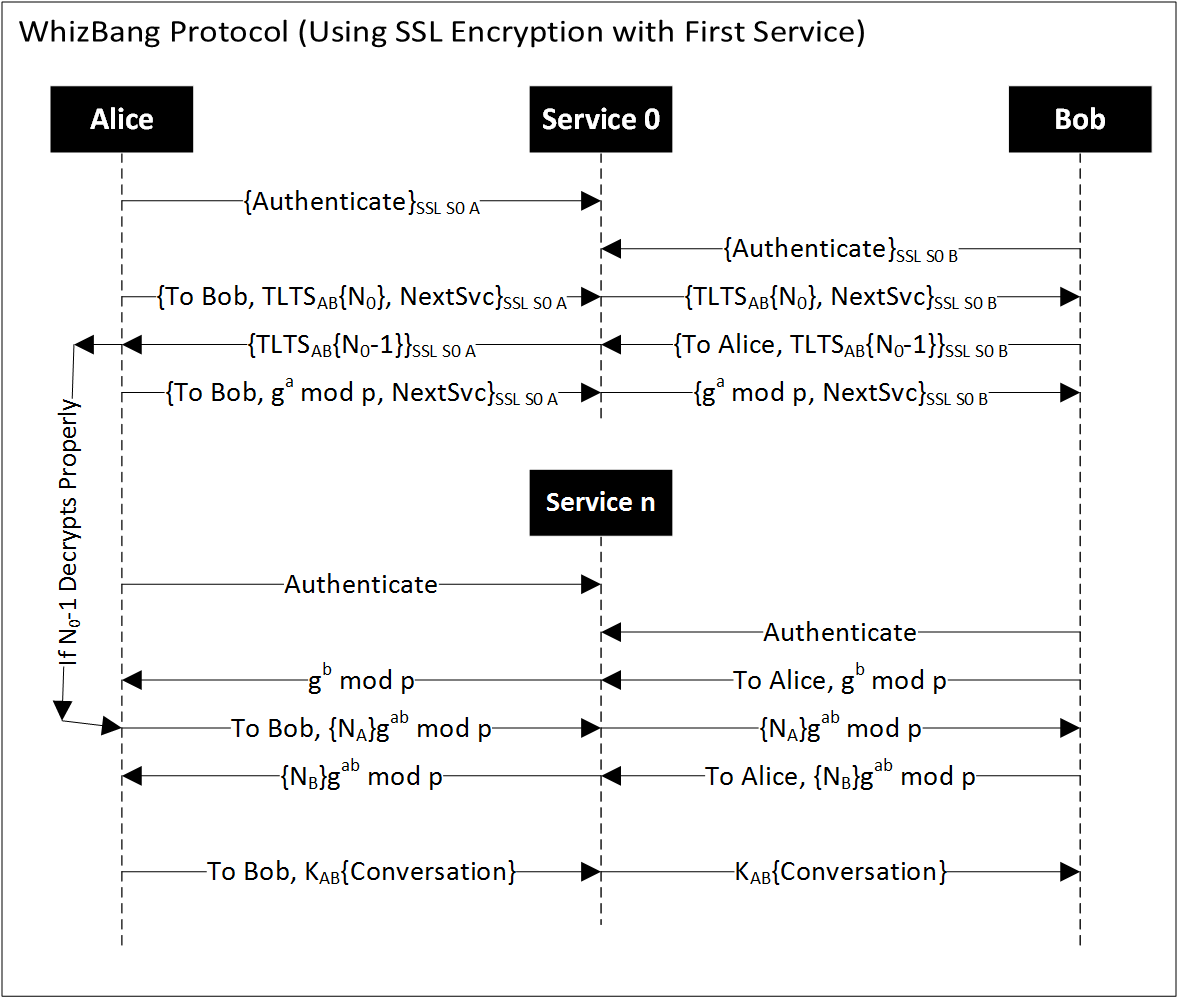
\includegraphics{ProtocolDiagramBW.png}

\section{Implementation}

\section{Conclusion}

\section{References}

\bibliographystyle{plain}
\bibliography{ProjectReport}

\end{multicols}
\end{document}